\documentclass[11pt]{article}
% Font tiếng việt
\usepackage{fontspec}
\usepackage[vietnamese]{babel}

% Sử dụng bảng dài có thể ngắt trang, bạn cần thêm 2 gói này vào preamble
\usepackage{longtable}
\usepackage{ragged2e}
\usepackage{hyperref}

\usepackage{graphicx}
\usepackage{amsmath, amssymb, amsfonts, bm}
\usepackage{xcolor}
\usepackage{hyperref}
\usepackage{pifont}
\newcommand{\xmark}{\ding{55}}
\newcommand{\cmark}{\ding{51}}
\usepackage{array}
\usepackage{float}

\definecolor{codehighlight}{rgb}{0.95,0.95,0.92} % Using your backcolour


\hypersetup{
    colorlinks=true,
    linkcolor=blue,
    filecolor=magenta,
    urlcolor=red,
    pdftitle={Overleaf Example},
    pdfpagemode=FullScreen,
}

\setmainfont{Times New Roman}
% \setsansfont{Arial} % Not used in the final layout, can comment out
% \setmonofont{Courier New} % Not used in the final layout, can comment out


% Page layout
\setlength{\topmargin}{-.5in}
\setlength{\textheight}{9.25in}
\setlength{\oddsidemargin}{0in}
\setlength{\textwidth}{6.8in}

% No explicit title formatting needed as we'll place it manually
\usepackage{titling}
\setlength{\droptitle}{-10em} % Keep this to prevent default title spacing issues if using \maketitle later for other purposes

\renewcommand{\maketitle}{%
    \begin{center}
        \fontsize{18}{20}\selectfont\textbf{Modul 3 Tuần 1 - Advanced Data Visualization}\\[1em]
        \fontsize{14}{16}\selectfont Time-Series Team\\[0.5em]
        \fontsize{14}{16}\selectfont Ngày 1 tháng 8 năm 2025
    \end{center}
    \vspace{1.5em} % Add some space after the custom title block
}


% Remove fancy header/footer as it's not in the image
% \usepackage{fancyhdr}
% \pagestyle{fancy}
% \fancyhf{}
% \renewcommand{\footrulewidth}{0.4pt}
% \lhead{\bfseries AI VIETNAM}
% \rhead{\bfseries aivietnam.edu.vn}
% \fancyfoot[C]{\thepage}

% Section format (không đánh số section) - Keep this
\usepackage{titlesec}
\titleformat{\section}
{\normalfont\Large\bfseries}
{}{0em}{}

% Listings (code block) - Keep this if you plan to use code blocks
\usepackage{listings}
\definecolor{codegreen}{rgb}{0,0.6,0}
\definecolor{codegray}{rgb}{0.5,0.5,0.5}
\definecolor{codepurple}{rgb}{0.58,0,0.82}
\definecolor{backcolour}{rgb}{0.95,0.95,0.92}
\lstdefinestyle{mystyle}{
    backgroundcolor=\color{backcolour},
    commentstyle=\color{codegreen},
    keywordstyle=\color{magenta},
    numberstyle=\tiny\color{codegray},
    stringstyle=\color{codepurple},
    basicstyle=\ttfamily\footnotesize,
    breaklines=true,
    captionpos=b,
    keepspaces=true,
    numbers=left,
    numbersep=5pt,
    tabsize=2,
    showspaces=false,
    showstringspaces=false,
    showtabs=false
}
\lstset{style=mystyle}


% Colored boxes
\usepackage[many]{tcolorbox}
\definecolor{lightgreenbox}{rgb}{0.85,0.95,0.85} % A light green color closer to the image
\newtcolorbox{summarybox}{
    colback = lightgreenbox,
    colframe = green!50!black, % A slightly darker green border
    boxsep = 5pt,
    arc = 4pt,
    outer arc = 4pt,
    boxrule = 0.5pt,
    left = 10pt,
    right = 10pt,
    top = 10pt,
    bottom = 10pt,
    % Add this line to ensure proper font encoding for Vietnamese characters
    fontupper = \setmainfont{Times New Roman}\normalfont,
}

% For math proofs or custom counters (tuỳ chọn nếu cần) - Can be removed if not used
\usepackage{lipsum}
\newcounter{mycounter}
\newcommand\showmycounter{\stepcounter{mycounter}\themycounter}
\newcommand\showlips{\stepcounter{mycounter}\lipsum[\value{mycounter}]}

% Others - Can be removed if not used
\usepackage{booktabs}
\usepackage{subcaption}
\usepackage{framed}
\usepackage{tikz}


%%%%%%%%%%%%%%%%%%%%%%%%%%%%%%%%%%%%%%%%%%%%%%%%%%%%%%%%%%%%%%%%%%%%%%%%%%%%%
%%%%%%%%%%%%%%%%%%%%%%%%%%%%%%%%%%%%%%%%%%%%%%%%%%%%%%%%%%%%%%%%%%%%%%%%%%%%%
%%%%%%%%%%%%%%%%%%%%%%%%%%%%%%%%%%%%%%%%%%%%%%%%%%%%%%%%%%%%%%%%%%%%%%%%%%%%%
\begin{document}

\maketitle % Call the redefined maketitle to display the custom title and date

\begin{summarybox}
    Buổi học thứ 6 (ngày 1/8/2025) được chia thành 4 phần chính nhằm giúp bạn hiểu được cách tìm đúng biểu đồ minh họa dựa trên 3 Case Study sử dụng Python.
    \begin{itemize}
        \item \textbf{Phần 1: Basic Data Visualization}
        \item \textbf{Phần 2 Case study: ETTH dataset}
        \item \textbf{Phần 3 Case study: Iris Dataset}
        \item \textbf{Phần 4 Case study: Student Performance}
    \end{itemize}
\end{summarybox}

\section{Phần 1: Basic Data Visualization}
Phần này đưa ra khung toàn diện để hiểu và áp dụng các kỹ thuật trực quan hóa dữ liệu cơ bản bằng Python, được tổ chức xoay quanh ba case study và hướng dẫn chọn biểu đồ.

\subsection{Giới thiệu các loại biểu đồ phổ biến}
Trước khi vào phần code, đây là giải thích chi tiết hơn về từng loại biểu đồ bạn sẽ gặp — cách hoạt động, khi nào dùng, điểm mạnh/nhược, và ví dụ nhỏ để minh hoạ.

\medskip
\noindent \textbf{1. Biểu đồ xu hướng (Trend / Time-series)}
\medskip
\textbf{Line Chart:} Line chart nối các điểm dữ liệu theo thứ tự (thường là thời gian). Dùng để nhận diện xu hướng chung, chu kỳ lặp, và các điểm đột biến (peaks/valleys).
\textit{Cách đọc:} nhìn dốc của đường để biết xu hướng (tăng/giảm), quan sát biên độ để thấy biến động.
\textit{Ưu điểm:} trực quan cho chuỗi thời gian, dễ so sánh nhiều series bằng nhiều đường.
\textit{Hạn chế:} với dữ liệu rời rạc không có thứ tự rõ ràng thì không phù hợp; nhiều đường quá sẽ gây rối.
\textit{Ví dụ:} nhiệt độ dầu trong ETTH theo giờ để thấy giờ đỉnh nhiệt.
\begin{figure}[H]
    \centering
    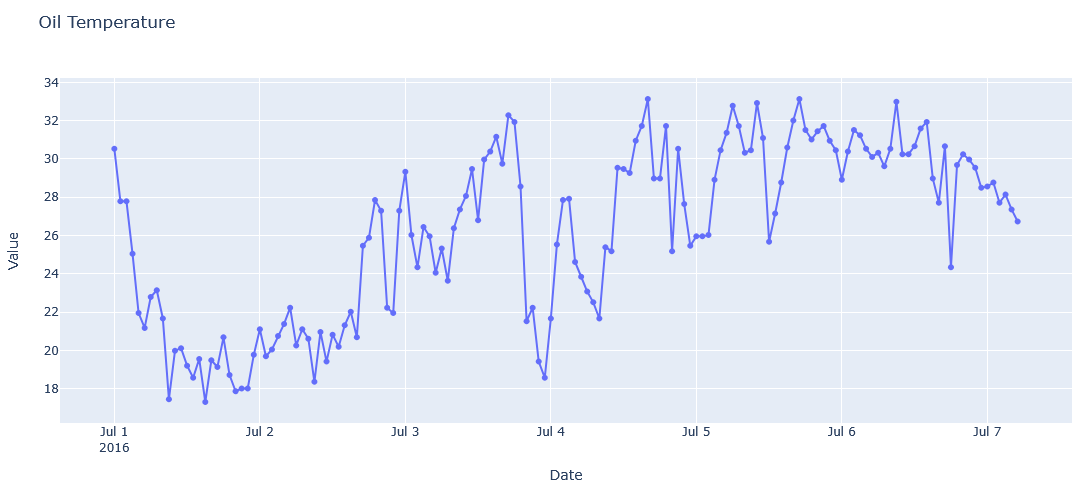
\includegraphics[width=0.4\linewidth]{images/lineC.png}
\end{figure}


\medskip
\noindent \textbf{2. Biểu đồ phân phối dữ liệu (Distribution)}

\medskip
\textbf{Histogram:} Chia dải giá trị liên tục thành các \textbf{bin} (khoảng/nhóm giá trị), sau đó hiển thị tần suất trong mỗi bin.
\textit{Ghi chú chuyên ngành:} \emph{bin} = một khoảng giá trị; số bin ảnh hưởng tới chi tiết/độ mượt của biểu đồ.
\textit{Ví dụ:} phân phối chiều dài cánh hoa trong Iris.
\begin{figure}[H]
    \centering
    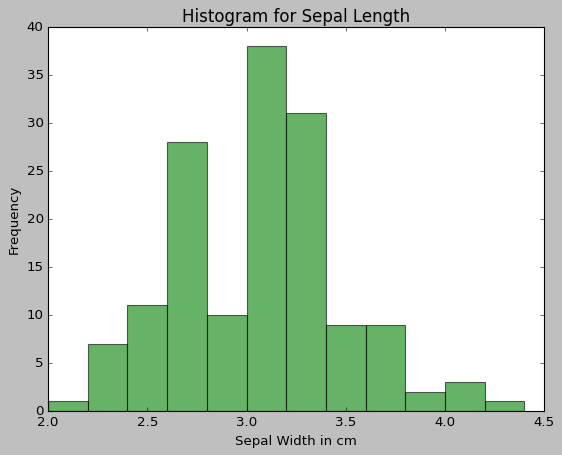
\includegraphics[width=0.4\linewidth]{images/Histogram.png}
\end{figure}

\medskip
\textbf{Box Plot (Hộp và râu):} Dùng để tóm tắt và trực quan hóa phân phối dữ liệu thông qua các phân vị (quartiles) và giá trị ngoại lai (outliers). Cấu tạo như sau:
\begin{figure}[H]
    \centering
    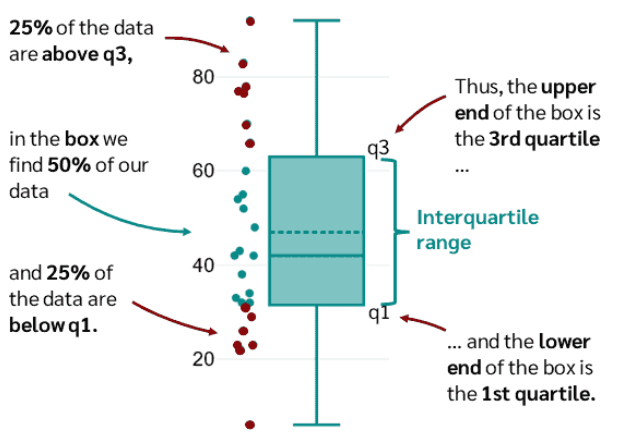
\includegraphics[width=0.5\linewidth]{images/boxplot_img.png}
\end{figure}
\begin{itemize}
    \item \textbf{Râu Đỉnh (Upper Whisker):} Giá trị lớn nhất nhưng không phải ngoại lai.
    \item \textbf{Râu Đáy (Lower Whisker):} Giá trị nhỏ nhất nhưng không phải ngoại lai.
    \item \textbf{Upper Part - Q3 (Upper Quartile):} 25\% dữ liệu lớn hơn giá trị này.
    \item \textbf{Median - Q2:} Giá trị trung vị, chia dữ liệu thành 2 nửa bằng nhau.
    \item \textbf{Lower Part - Q1 (Lower Quartile):} 25\% dữ liệu nhỏ hơn giá trị này.
    \item \textbf{Outlier:} Các điểm bất thường, được định nghĩa là nhỏ hơn $Q_{1} - 1.5 \times IQR$ hoặc lớn hơn $Q_{3} + 1.5 \times IQR$.
\end{itemize}

\noindent \textbf{IQR (Interquartile Range):} Là khoảng giữa Q1 và Q3, công thức:
\[
IQR = Q_{3} - Q_{1}
\]
$\rightarrow$ thể hiện trực quan 50\% dữ liệu tập trung ở giữa (middle 50\%).

\medskip
\textbf{Ví dụ minh họa:} Với dãy dữ liệu \([5, 7, 8, 12, 14, 18, 21, 23, 24, 26, 30]\):
\begin{itemize}
    \item Median (Q2) = 18
    \item Lower half = \([5, 7, 8, 12, 14]\) $\Rightarrow$ Q1 = 8
    \item Upper half = \([21, 23, 24, 26, 30]\) $\Rightarrow$ Q3 = 24
    \item $IQR = Q_{3} - Q_{1} = 24 - 8 = 16$
    \item \textbf{Upper Bound:} $Q_{3} + 1.5 \times IQR = 24 + 24 = 48$
    \item \textbf{Lower Bound:} $Q_{1} - 1.5 \times IQR = 8 - 24 = -16$
\end{itemize}

\noindent Vì toàn bộ dữ liệu đều nằm trong khoảng \([-16, 48]\), nên không có ngoại lai trong ví dụ này.
Minh họa khác sử dụng Boxplot để kiểm tra giá trị ngoại lai và phân bổ giá trị của từng Lớp giá trị.

\begin{figure}[H]
    \centering
    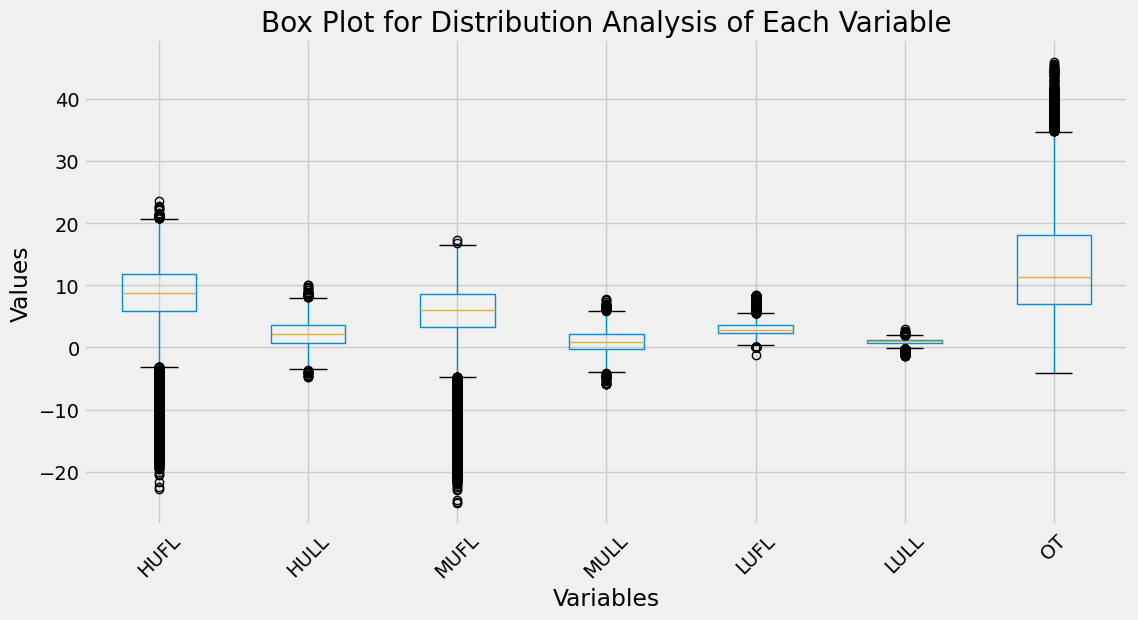
\includegraphics[width=0.5\linewidth]{images/BoxP.png}
\end{figure}


\medskip
\textbf{KDE Plot:} KDE = \emph{Kernel Density Estimate} (ước lượng mật độ bằng kernel), là một cách mượt hoá histogram để ước lượng mật độ xác suất liên tục.
\textit{Ghi chú chuyên ngành:} \emph{bandwidth} (băng thông) điều chỉnh mức mượt — nhỏ quá gây nhiễu, lớn quá che đi chi tiết.
\textit{Ví dụ:} mật độ chiều dài cánh hoa theo loài.
\begin{figure}[H]
    \centering
    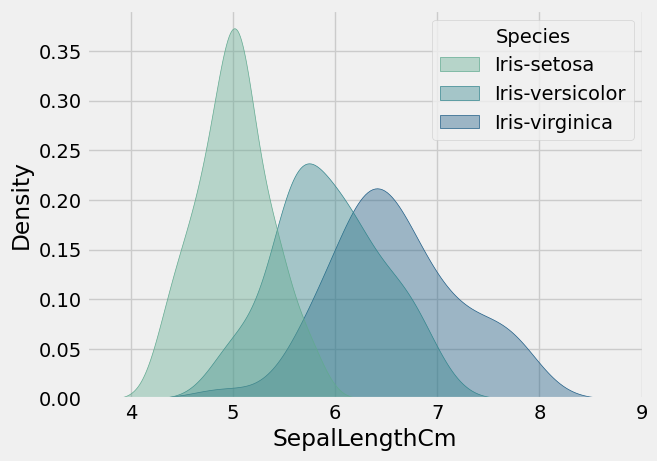
\includegraphics[width=0.4\linewidth]{images/KernelDensityEstimate_Plot.png}
\end{figure}


\textbf{Distribution / DistPlot:} Kết hợp histogram và KDE (và đôi khi \emph{rug plot}) để đồng thời thấy tần suất và mật độ.
\textit{Ghi chú chuyên ngành:} \emph{rug plot} = các dấu nhỏ trên trục x để chỉ từng quan sát; hữu ích để thấy mật độ thô.
\begin{figure}[H]
    \centering
    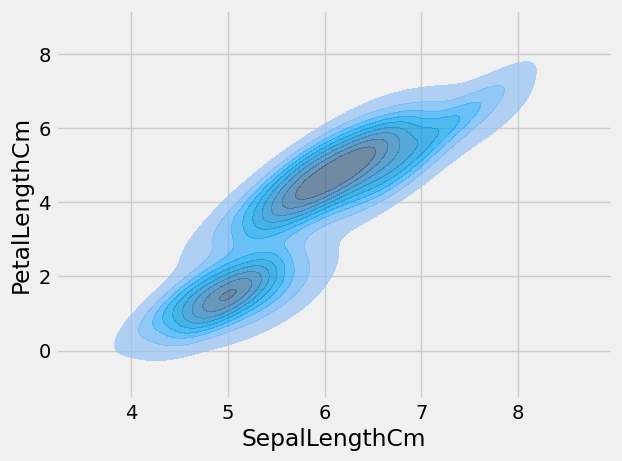
\includegraphics[width=0.4\linewidth]{images/Displot.png}
\end{figure}


\medskip
\noindent \textbf{3. Biểu đồ so sánh nhóm (Comparison)}
\medskip
\textbf{Bar Chart:} Mỗi cột biểu diễn giá trị (tổng, trung bình, tỷ lệ) cho một nhóm rời rạc.
\textit{Ghi chú chuyên ngành:} có thể thêm \emph{error bars} (thanh sai số) để thể hiện độ tin cậy/độ biến thiên.
\textit{Ví dụ:} doanh số theo từng chi nhánh.
\begin{figure}[H]
    \centering
    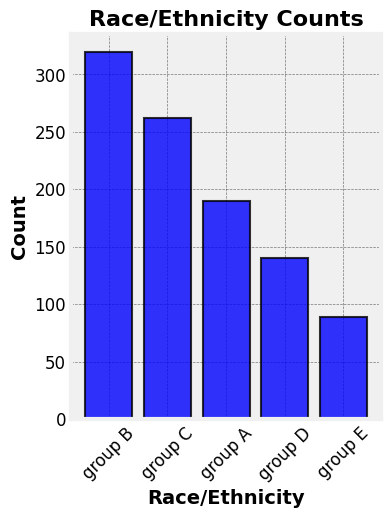
\includegraphics[width=0.3\linewidth]{images/BarC.png}
\end{figure}

\medskip
\textbf{Count Plot:} Là bar chart chuyên cho biến phân loại, hiển thị tần suất từng nhãn. Dùng để kiểm tra cân bằng lớp (class balance).
\textit{Ví dụ:} số sinh viên theo nhóm ôn luyện/không ôn luyện.
\begin{figure}[H]
    \centering
    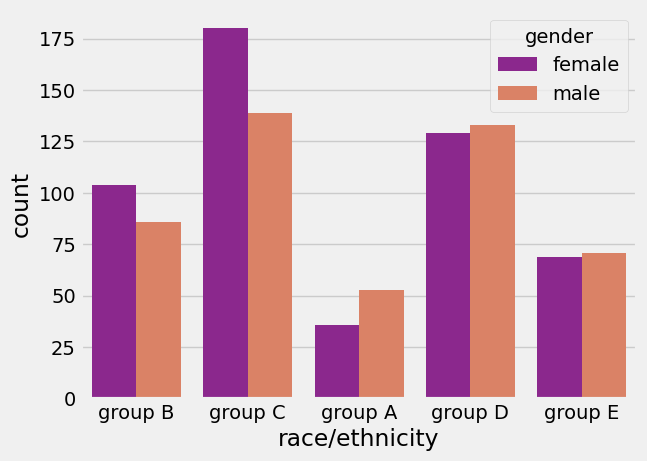
\includegraphics[width=0.3\linewidth]{images/CountPlots.png}
\end{figure}

\medskip
\textbf{Stacked Bar Chart:} Mỗi cột chia thành các phần con (các lớp nhỏ trong nhóm).
\textit{Ghi chú chuyên ngành:} \emph{normalized stacked bar} = chuẩn hoá theo phần trăm để so sánh cấu trúc (tỉ lệ) giữa các nhóm.
\textit{Ví dụ:} doanh số online vs offline theo tháng.
\begin{figure}[H]
    \centering
    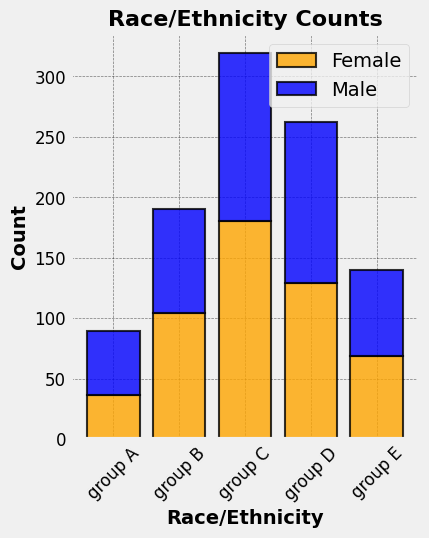
\includegraphics[height=0.4\textheight]{images/stackedBarC.png}
\end{figure}

\medskip
\noindent \textbf{4. Biểu đồ quan hệ giữa các biến (Relationship)}

\medskip
\textbf{Scatter Plot:} Mỗi điểm là một cặp (x, y), dùng để phát hiện xu hướng, cluster (cụm), và outlier.
\textit{Ghi chú chuyên ngành:} \emph{overplotting} = hiện tượng chồng điểm khi có quá nhiều điểm; xử lý bằng \emph{alpha/transparency} (độ trong suốt), \emph{jitter} (dời nhẹ điểm) hoặc \emph{hexbin} (đếm mật độ trong ô lục giác). \emph{Trendline/regression} = đường ước lượng mối quan hệ (dùng để định lượng).
\textit{Ví dụ:} thời gian giao hàng vs tỷ lệ huỷ đơn.
\begin{figure}[H]
    \centering
    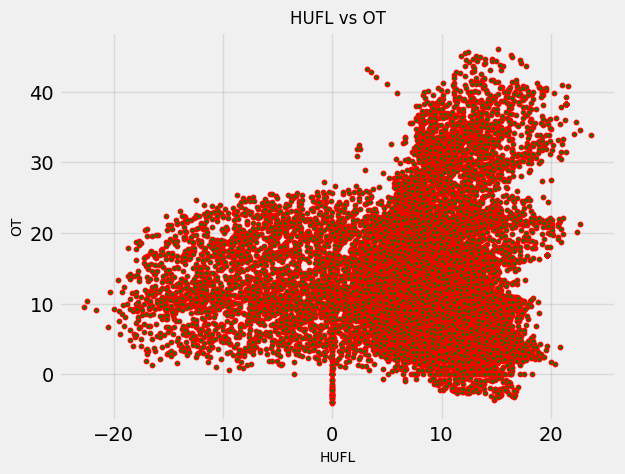
\includegraphics[width=0.5\linewidth]{images/ScatterC.png}
\end{figure}


\medskip
\textbf{Bubble Chart:} Scatter mở rộng thêm biến thứ ba qua kích thước bong bóng (size).
\textit{Ghi chú chuyên ngành:} cần \emph{scale} (chuẩn hoá) kích thước để tránh hiểu nhầm về diện tích.
\textit{Ví dụ:} doanh thu (y), số đơn (x), thị phần (kích thước).
\begin{figure}[H]
    \centering
    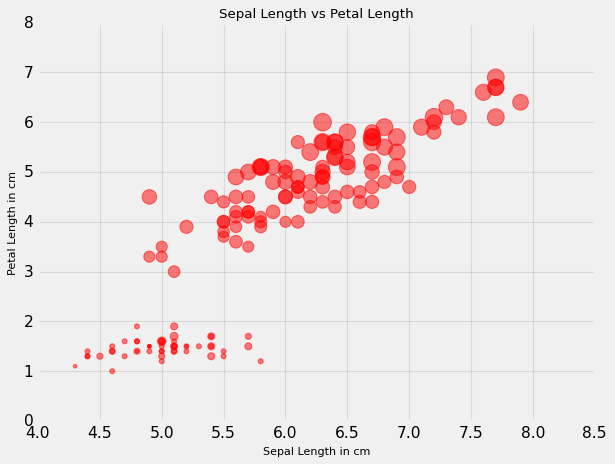
\includegraphics[width=0.5\linewidth]{images/BubbleP.png}
\end{figure}

\medskip
\textbf{Interactive Scatter (Plotly):} Scatter hỗ trợ tương tác (hover = di chuột xem chi tiết, zoom, lọc). Hữu ích khi khám phá dữ liệu lớn hoặc trình bày cho người dùng tương tác.
\textit{Ví dụ:} bản đồ pickup Uber với tooltip chi tiết.
\begin{figure}[H]
    \centering
    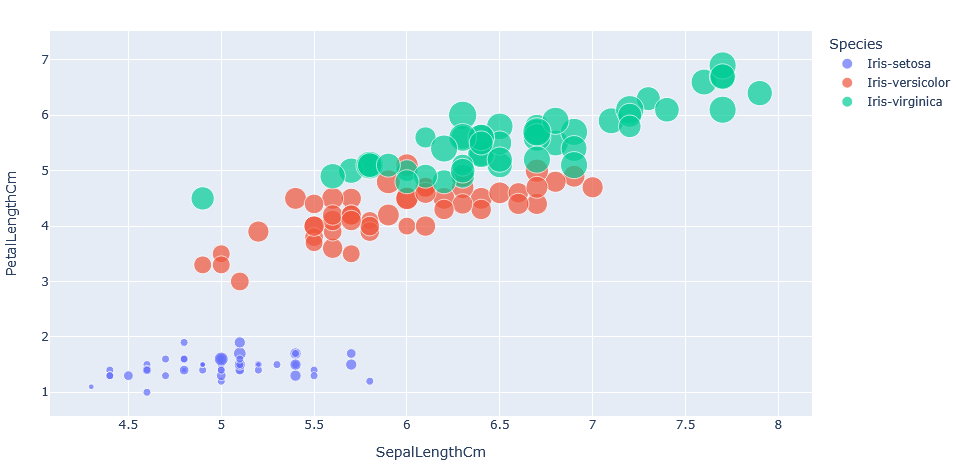
\includegraphics[width=0.6\linewidth]{images/PlottyScatter.png}
\end{figure}

\medskip
\textbf{Pair Plot (Scatter matrix):} Ma trận scatter cho mọi cặp biến, kèm biểu đồ phân phối (histogram/KDE) trên đường chéo; tiện để rà soát mối quan hệ cặp đôi và phân biệt nhóm theo \emph{hue} (màu phân nhóm).
\textit{Ghi chú chuyên ngành:} \emph{hue} = biến dùng để tô màu điểm theo nhóm.
\textit{Ví dụ:} 4 đặc trưng Iris để quan sát sự tách biệt giữa các loài.
\begin{figure}[H]
    \centering
    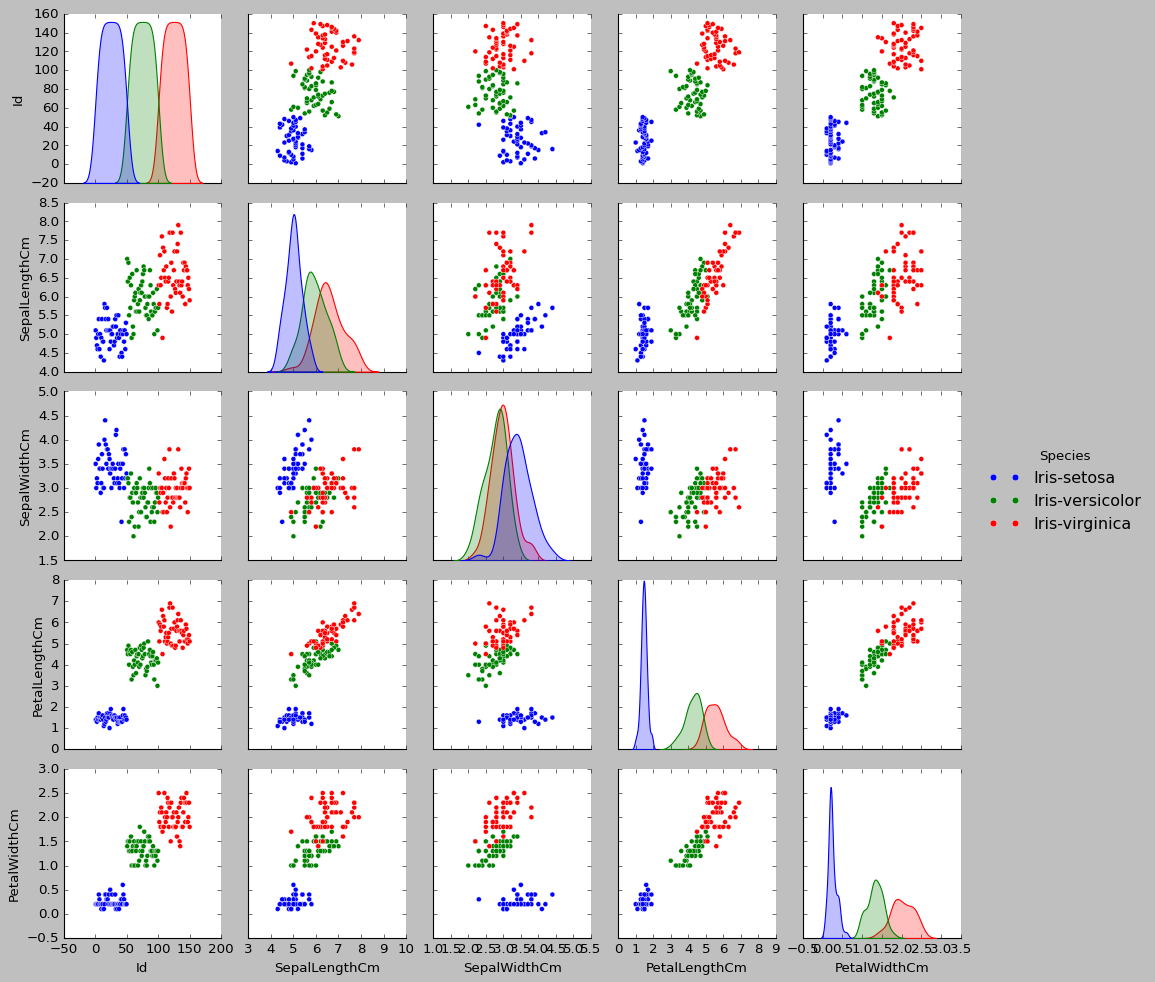
\includegraphics[width=0.7\linewidth]{images/PairP_Iris.png}
\end{figure}
\begin{figure}[H]
    \centering
    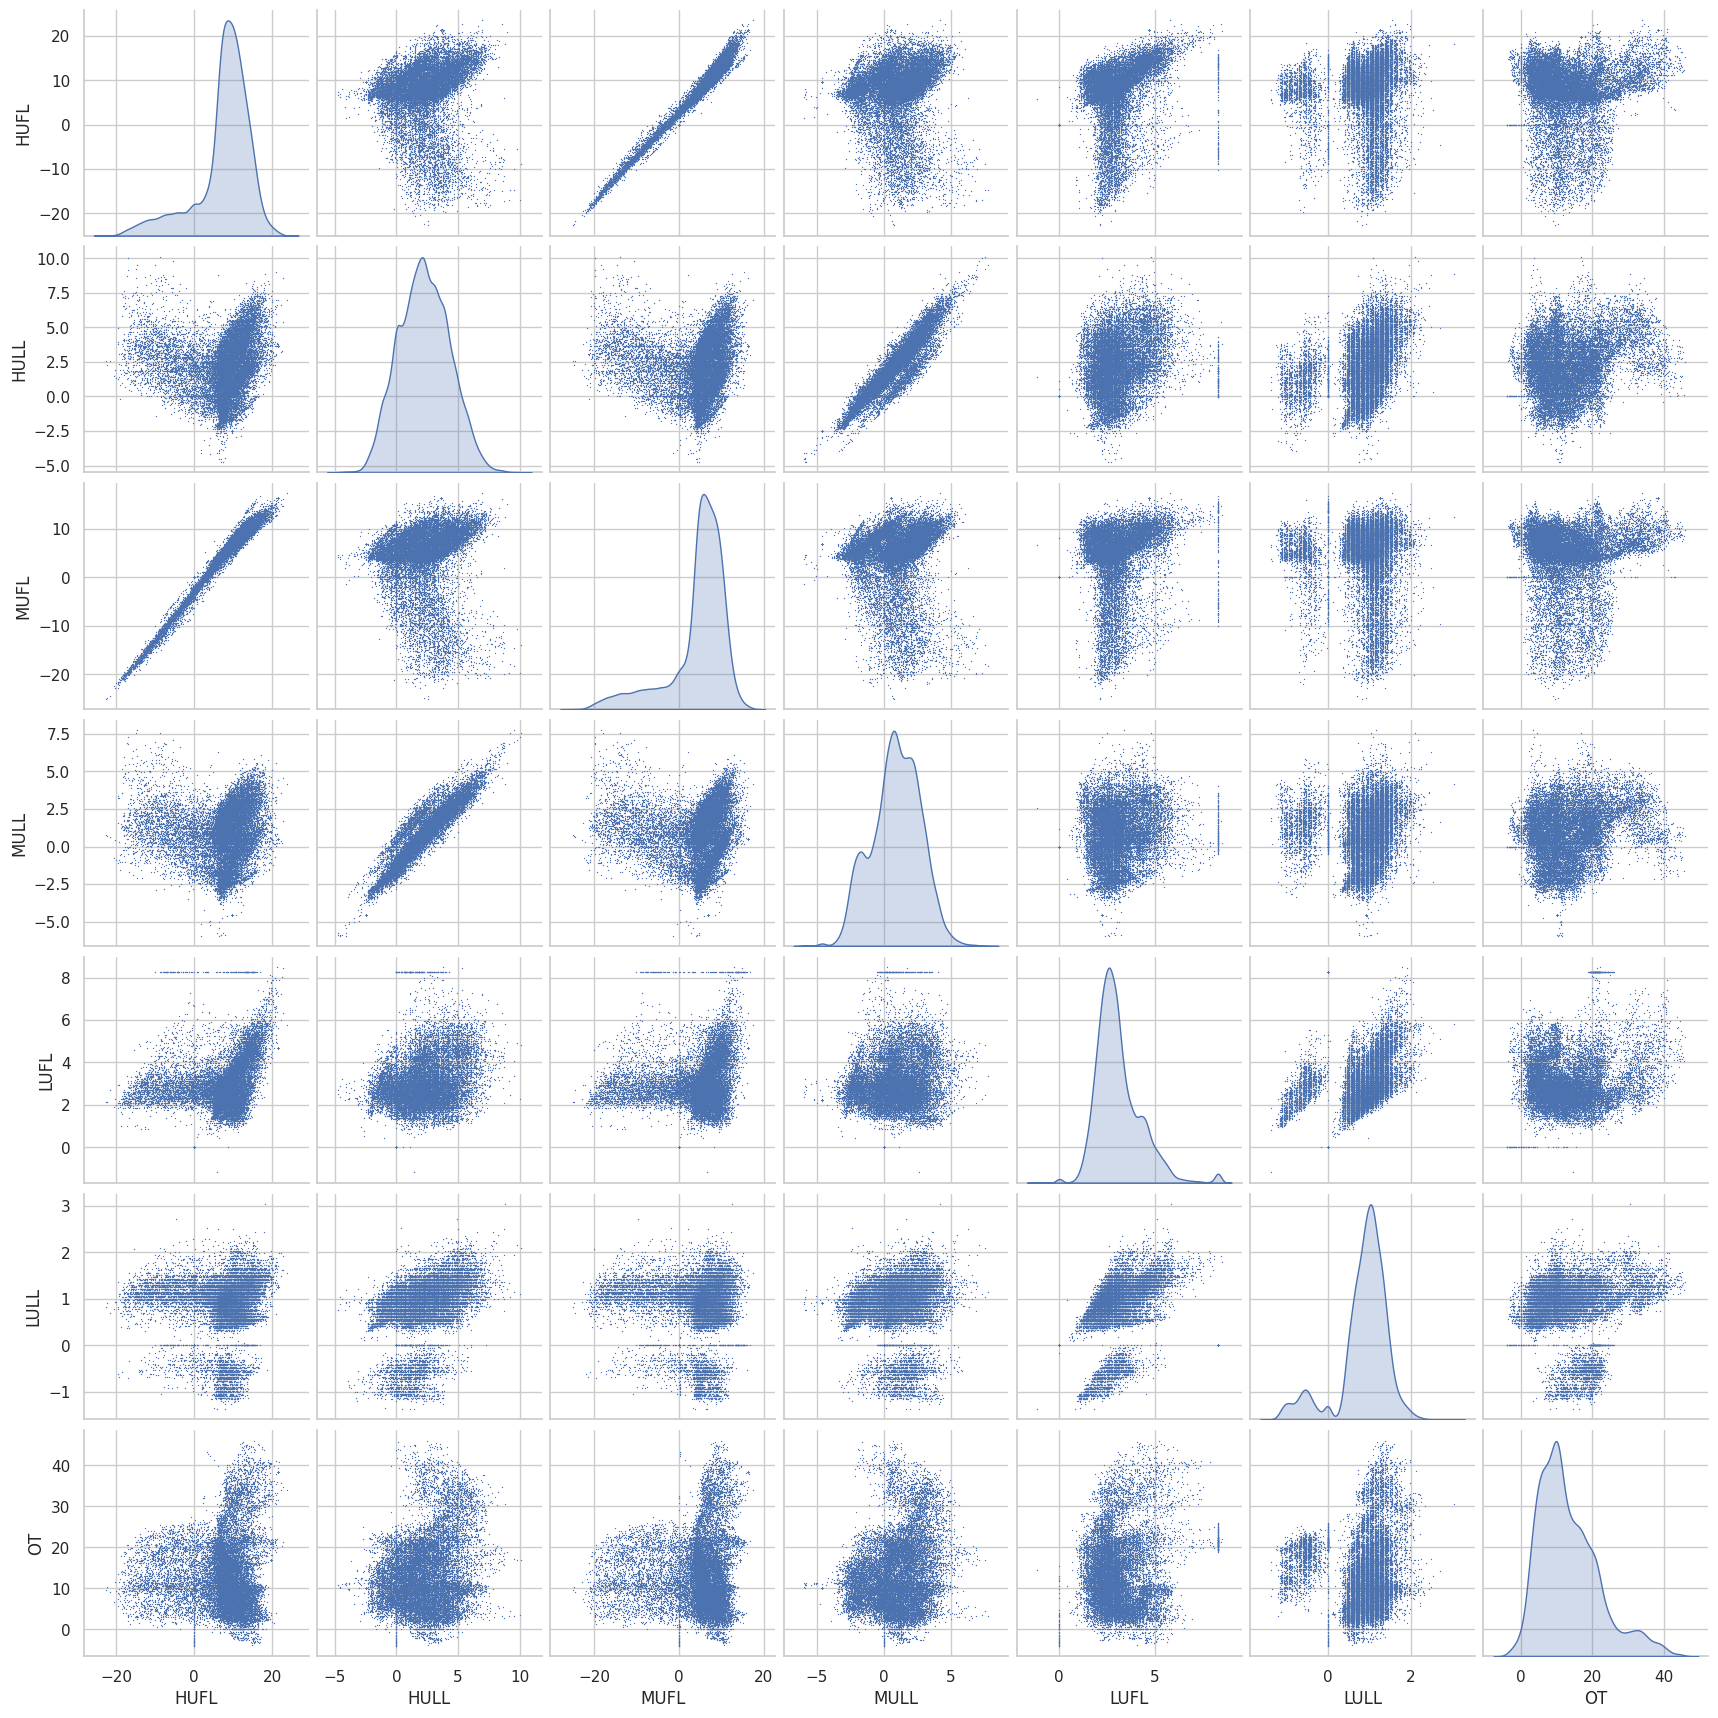
\includegraphics[width=0.7\linewidth]{images/PairPlot_dots.png}
\end{figure}


\medskip
\noindent \textbf{5. Biểu đồ thành phần - tổng thể (Part-to-Whole)}
\medskip
\textbf{Pie Chart:} Hiển thị tỷ lệ phần trăm các phần trong tổng thể; dùng khi số phần nhỏ (thường <7).
\textit{Ghi chú chuyên ngành:} tránh lát mảnh quá nhỏ, luôn thêm nhãn phần trăm hoặc legend để người đọc dễ hiểu.
\textit{Ví dụ:} tỷ lệ tải HUFL/MUFL/LUFL.
\begin{figure}[H]
    \centering
    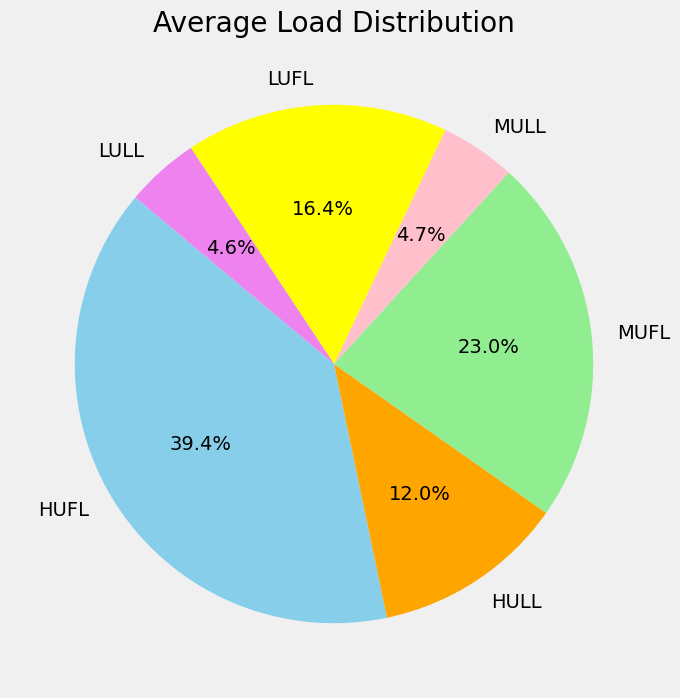
\includegraphics[width=0.5\linewidth]{images/PieC.png}
\end{figure}

\medskip
\noindent \textbf{6. Biểu đồ đặc biệt}

\medskip
\textbf{Heatmap:} Ma trận màu (color matrix) hiển thị giá trị theo hai chiều — thường dùng cho ma trận tương quan hoặc bản đồ mật độ. Giúp nhanh nhận diện \emph{hotspot} (vùng giá trị cao).
\textit{Ví dụ:} ma trận tương quan giữa các cảm biến ETTH.
\begin{figure}[H]
    \centering
    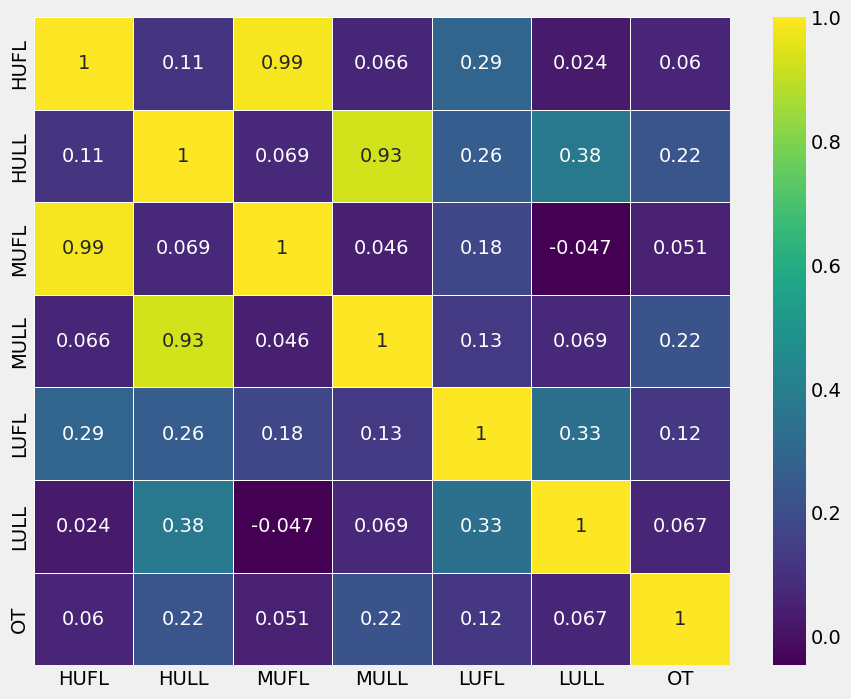
\includegraphics[width=0.5\linewidth]{images/heatmap.png}
\end{figure}

\medskip
\textbf{Word Cloud:} Vẽ từ theo kích thước tương ứng tần suất hoặc trọng số; hữu ích cho khám phá nhanh các từ khóa nổi bật trong dữ liệu văn bản.
\textit{Ghi chú chuyên ngành:} trước khi tạo, cần loại bỏ \emph{stopwords} (từ dừng — các từ phổ biến không mang ý nghĩa như "và", "là"), và cân nhắc \emph{stemming/lemmatize} (rút gốc từ) để nhóm các dạng từ tương tự.
\textit{Ví dụ:} từ khoá tìm kiếm nhiều nhất trên YouTube.
\begin{figure}[H]
    \centering
    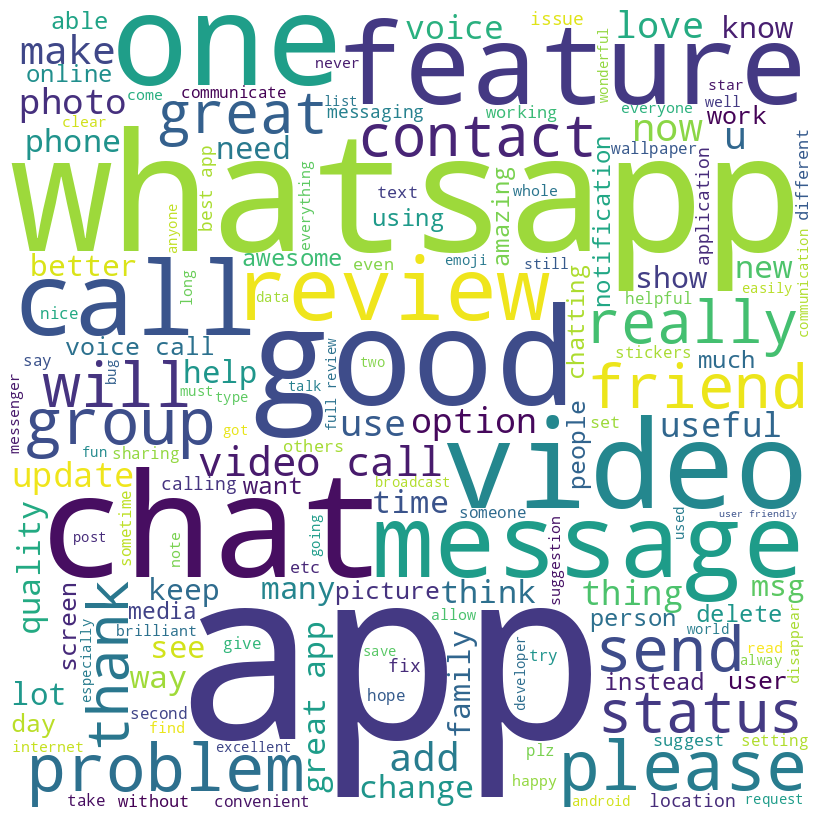
\includegraphics[width=0.5\linewidth]{images/WordCloud.png}
\end{figure}

Để hiểu rõ hơn về code của từng biểu đồ, hãy truy cập: \href{https://drive.google.com/file/d/1BkQBikJYrhgLE_gemTrOTmcgx8GPVUrS/view?usp=sharing}{Code Visualization}


\subsection{Giới thiệu quy trình chọn biểu đồ}
Khi bắt đầu trực quan hóa dữ liệu, có hai câu hỏi quan trọng cần đặt ra: \\
\textbf{(1)} Thông tin hay vấn đề nào cần minh họa? \\
\textbf{(2)} Loại biểu đồ nào thể hiện rõ nhất thông tin đó? Việc lựa chọn đúng phụ thuộc vào loại dữ liệu, mối quan hệ giữa các biến, mục tiêu trực quan hóa và đối tượng người xem. Không có một biểu đồ duy nhất phù hợp cho tất cả trường hợp, do đó đôi khi cần thử nghiệm nhiều loại khác nhau để tìm lựa chọn tối ưu.

\begin{figure}[H]
    \centering
    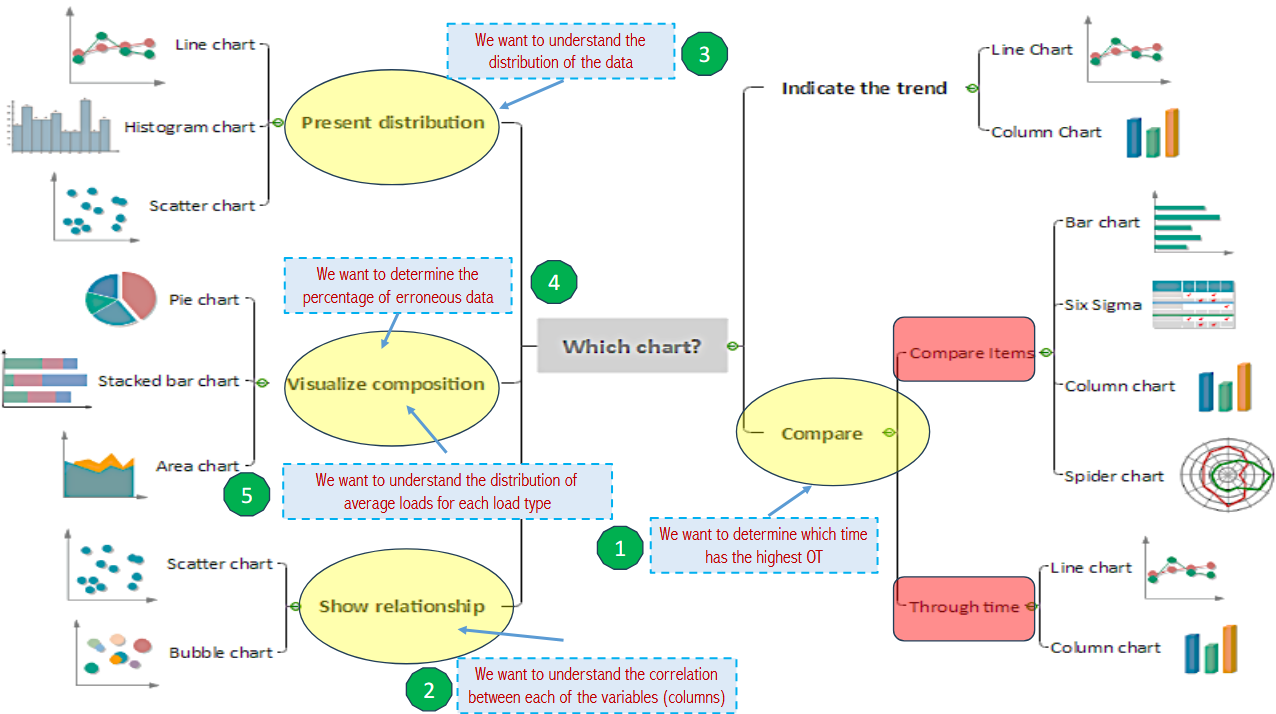
\includegraphics[width=0.9\linewidth]{images/graph_to_choose_whichChart.png}
    \caption{Nguyên tắc chọn loại biểu đồ}
    \label{fig:which chart}
\end{figure}

Quy trình chọn biểu đồ có thể đi theo các bước sau:
\begin{itemize}
    \item Bước 1: Xác định loại dữ liệu $\rightarrow$ dữ liệu định lượng (số đo, tính toán), dữ liệu phân loại (ví dụ Yes/No, Nam/Nữ), dữ liệu chuỗi thời gian (time series), hoặc dữ liệu không gian (gắn với vị trí địa lý).
    \begin{figure}[H]
        \centering
        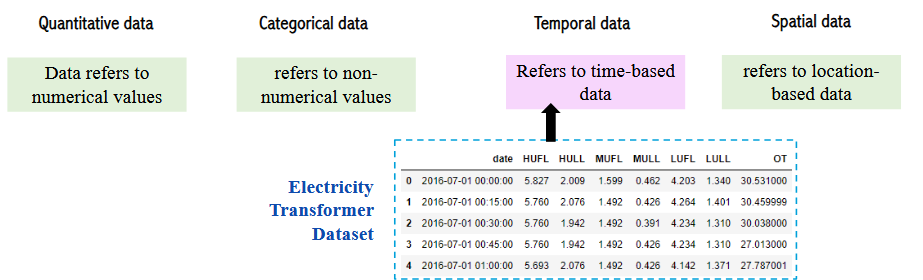
\includegraphics[width=1\linewidth]{images/rc1.png}
        \label{fig:rc1}
    \end{figure}

    \item Bước 2: Xác định thông tin muốn truyền tải $\rightarrow$ nếu cần thể hiện xu hướng theo thời gian thì dùng line chart hoặc area chart (ví dụ: mức tiêu thụ điện trong một ngày). Nếu cần so sánh giữa các nhóm thì dùng bar chart hoặc column chart. Nếu muốn xem phân phối dữ liệu thì dùng histogram hoặc box plot.
    \begin{figure}[H]
        \centering
        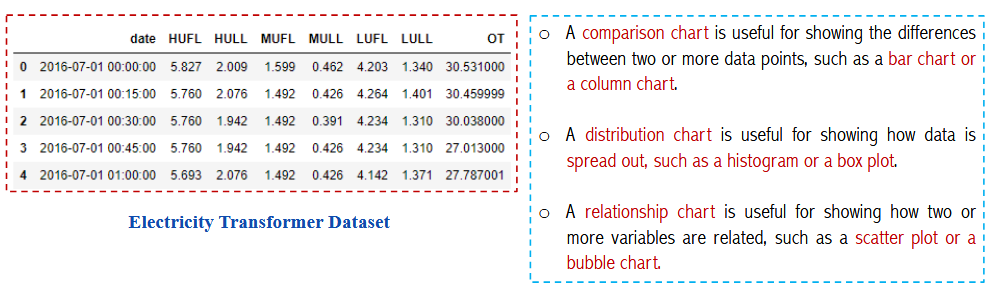
\includegraphics[width=1\linewidth]{images/rc2.png}
        \label{fig:rc2}
    \end{figure}

    \item Bước 3: Xác định mục tiêu trực quan hóa $\rightarrow$ bạn muốn làm nổi bật xu hướng, phân phối, hay mối quan hệ giữa các biến?
    \begin{figure}[H]
        \centering
        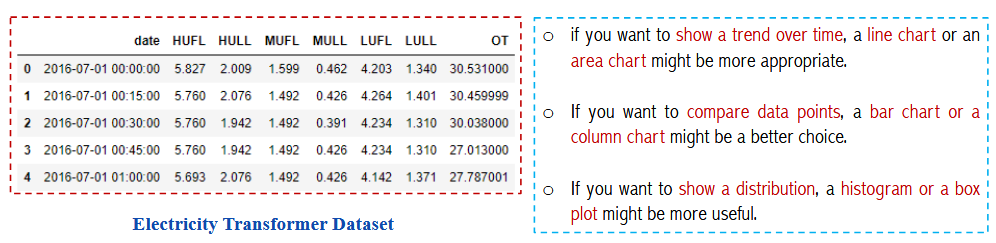
\includegraphics[width=1\linewidth]{images/rc3.png}
        \label{fig:rc3}
    \end{figure}

    \item Bước 4: Xác định đối tượng người xem $\rightarrow$ nếu đối tượng là chuyên gia có thể dùng biểu đồ phức tạp (heatmap, scatter matrix), còn với công chúng thì nên chọn biểu đồ trực quan, dễ hiểu (bar chart, pie chart).
    \begin{figure}[H]
        \centering
        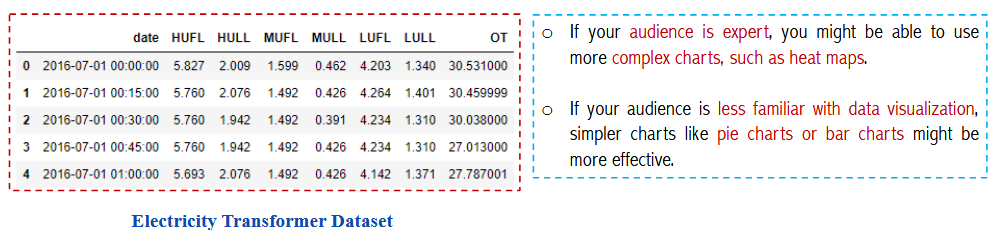
\includegraphics[width=1\linewidth]{images/rc4.png}
        \label{fig:rc4}
    \end{figure}

    \item Bước 5: Chọn loại biểu đồ phù hợp $\rightarrow$ thử nghiệm nhiều biểu đồ khác nhau và so sánh để chọn cách thể hiện hiệu quả nhất, vì không có giải pháp “one-size-fits-all”.
    \begin{figure}[H]
        \centering
        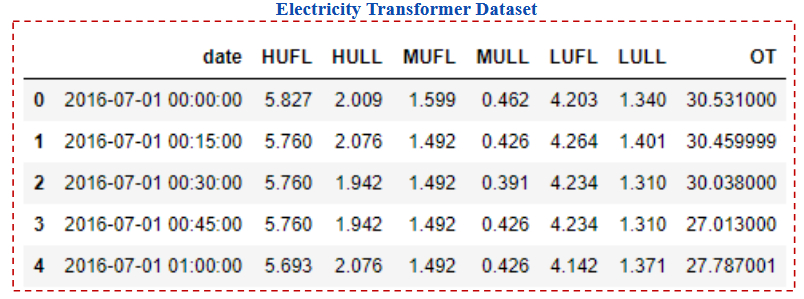
\includegraphics[width=1\linewidth]{images/rc5.png}
        \label{fig:rc5}
    \end{figure}

\end{itemize}


\section{Phần 2: Case Study ETTH Dataset}
\subsubsection*{Ví dụ: ETTH Dataset (Time Series)}
Với bộ dữ liệu ETTH, mục tiêu là tìm ra thời điểm mức tiêu thụ điện cao nhất. Quy trình phân tích đi theo: xác định mục tiêu $\rightarrow$ tìm mối quan hệ giữa các biến (nhiệt độ dầu, tải máy biến áp) $\rightarrow$ kiểm tra phân phối dữ liệu để phát hiện bất thường $\rightarrow$ đánh giá tỷ lệ dữ liệu lỗi hoặc thiếu. Kết quả giúp lựa chọn biểu đồ line chart cho xu hướng, box plot để xem phân phối, và correlation chart để phân tích mối quan hệ giữa biến.


\subsection{Chuẩn bị dữ liệu}
Tải dữ liệu và tính các thống kê cơ bản (số lượng, trung bình, độ lệch chuẩn, phần trăm vị trí) để đánh giá chất lượng và phân phối dữ liệu.

\subsection{Mục tiêu trực quan hóa}
\begin{itemize}
    \item Xác định thời điểm nhiệt độ dầu đạt đỉnh.
    \item Hiểu mối tương quan giữa các biến.
    \item Phân tích phân phối dữ liệu và phát hiện dữ liệu sai lệch.
    \item Đánh giá phân phối tải (HUFL, MUFL, LUFL).
\end{itemize}

\subsection{Các loại biểu đồ sử dụng}
\begin{itemize}
    \item \textbf{Line chart:} Trực quan hóa xu hướng và chuỗi thời gian (ví dụ: nhiệt độ dầu, loại tải).
    \item \textbf{Box plot:} Thể hiện phân phối dữ liệu, ngoại lai và giá trị trung tâm.
    \item \textbf{Bar chart và Pie chart:} Biểu diễn dữ liệu phân loại và tỷ lệ giữa các loại tải.
    \item \textbf{Donut chart và Correlation chart:} Thể hiện quan hệ phần-toàn bộ và mối tương quan giữa các biến.
\end{itemize}


\section{Phần 3: Case Study Iris Dataset}
Bộ dữ liệu Iris – kinh điển trong học máy – cho thấy các kỹ thuật trực quan hóa nâng cao cho dữ liệu liên tục và đa biến.

\subsection{Tổng quan dữ liệu}
Chứa các thông số đo của hoa iris theo loài, cho phép phân tích mối quan hệ giữa các biến số.

\subsection{Các trực quan sử dụng}
\begin{itemize}
    \item \textbf{Histogram:} Thể hiện phân phối tần suất và độ lệch (ví dụ: chiều dài cánh hoa, chiều rộng đài hoa).
    \item \textbf{Scatter plot:} Phân tích mối quan hệ cặp, chỉ ra kiểu tương quan.
    \item \textbf{Bubble chart:} Thêm biến thứ ba bằng kích thước bong bóng, phục vụ phân tích đa chiều.
    \item \textbf{KDE plot:} Minh họa mật độ xác suất cho phân phối đơn biến và nhị biến.
    \item \textbf{Displot chart:} Kết hợp histogram và KDE để có cái nhìn bổ sung về phân phối.
    \item \textbf{Biểu đồ 3D:} Thể hiện quan hệ giữa ba biến để phân tích phụ thuộc phức tạp.
\end{itemize}

\textbf{Tóm tắt:} Case study này làm nổi bật cách nhiều loại biểu đồ khác nhau giúp tăng khả năng diễn giải và khám phá insight.


\subsection{Kỹ thuật trực quan hóa}
\begin{itemize}
    \item \textbf{Bar chart:} Thể hiện sự thay đổi rời rạc giữa các nhóm (ví dụ: giới tính, học vấn của phụ huynh, việc chuẩn bị ôn thi).
    \item \textbf{Count plot:} Hiển thị tần suất xuất hiện của biến phân loại để xác định nhóm chiếm ưu thế hoặc xu hướng.
\end{itemize}

\textbf{Tóm tắt:} Các trực quan hóa này giúp phát hiện yếu tố ảnh hưởng đến kết quả học tập, hỗ trợ các biện pháp giáo dục có mục tiêu.

\section{Ôn tập: Cách chọn biểu đồ phù hợp}
\begin{enumerate}
    \item Xác định loại dữ liệu: định lượng, phân loại, chuỗi thời gian, hoặc không gian.
    \item Xác định quan hệ giữa các biến: so sánh, phân phối, quan hệ.
    \item Xác định mục tiêu trực quan hóa: xu hướng, so sánh, phân phối.
    \item Xác định đối tượng: chuyên gia (heatmap) hay công chúng (pie, bar).
    \item Thử nghiệm nhiều loại biểu đồ để chọn lựa phù hợp nhất.
\end{enumerate}

\section{Lời Kết}
Dữ liệu số là cho máy còn hình ảnh trực quan từ dữ liệu là cho mình. Để hiểu cách máy hoạt động như thế nào, để nhận viết được mối quan hệ trong đời sống thực tế có thể là thời gian đi học và thời gian tắc đường hoặc hành vi mua hàng đến yếu tố làm giao động cổ phiếu. DÙ cho gì đi nữa, thì team TimeSeries cũng tin rằng chỉ với trực quan hóa, con người mới có thể thực sự hiểu những con số mà mình vận dụng.

\end{document}
